\section{Numerical quadratures}
Methods for integrating $f(x)$ on the interval $[a,b]$, using $m$ points. The used variable $c$ is always contained in this interval.
%Formulas for the most basic Newton-Cotes quadratures, at least trapezoid and mid-point. 

\subsection{Composite Trapezoid Rule}
$$
\int_{a}^{b} f(x) \diff{x} = \frac{h}{2}(y_0+y_m + 2\sum_{i=1}^{m-1}y_i) - \frac{(b-a)h^2}{12}f''(c),
$$
where $h = (b-a)/m$.

\subsection{Composite Midpoint Rule}
Functions with removable singularities at an interval endpoint can be handled with
$$
\int_{a}^{b} f(x) \diff{x} = h \sum_{i=1}^mf(w_i) + \frac{(b-a)h^2}{24}f''(c),
$$
where $h = (b - a)/m$. The $w_i$ are the midpoints of $m$ equal subintervals of $[a,b]$.

\subsection{Higher order quadratures}
%Connection between interpolation and quadratures (this way one can e.g. derive Simpson's rule on an interval). Construction of composite quadratures from quadratures on one interval (remember the idea, not the formulas). 

% Simpson's: Degree 2 NCF, 3 terms, Degree 2 polynomial, x_0 to x_2

To find the Newton-Cotes quadrature of the $n$th degree, use the Lagrange polynomial of the $n$th degree with its interpolation error term given above
$$
\int_{x_0}^{x_n} f(x) \diff{x} = \int_{x_0}^{x_n} P_{n}(x) + E_n(x) \diff{x}, 
$$
where
$$
\int_{x_0}^{x_n} P_{n} = \sum_{i=0}^n f(x_i) \int_{x_0}^{x_n} L_k(x) \diff{x}.
$$

The degree of precision is $n$ (for $n$ odd) and $n+1$ (for $n$ even), with $n+1$ function evaluations.
%%TODO: Check if I havent fucked up the endpoints etc. Derive Simpson's method with these rules, and see if I get the correct formula

\subsection{Gaussian quadrature}
%Idea of orthogonal polynomials (do not memorize the formulas, but how the polynomials can be derived) and associated quadratures (goes back to the connection between quadratures and interpolation).

\begin{definition}
The set of nonzero functions $\{p_0,...,p_n\}$ on the interval $[a,b]$ is \textbf{orthogonal} on $[a,b]$ if
$$
\int_a^b p_j(x)p_k(x)dx = \\
\begin{cases}
    0 & j \neq k \\
    \neq 0 & j = k
\end{cases}
$$
\end{definition}

\begin{theorem}
These orthogonal polynomials, where deg $p_i = i$, form a basis for the vector space of degree at most $n$ polynomials on $[a,b]$. $p_i$ then has $i$ distinct roots in the interval $(a,b)$.
\end{theorem}

The set of \textbf{Legendre polynomials}
$$
p_i(x) = \frac{1}{2^i i!}\frac{\diff{}^i}{\diff{x}î}[(x^2-1)^i], \text{ for } 0 \leq i \leq n
$$
is orthogonal on $[-1,1]$. 
\vspace{2mm}
\newline
Gaussian quadrature of the $n$th degree is derived from integrating an interpolating polynomial of $f(x)$ whose nodes are the Legendre roots of $p_n$.

$$
\int_{-1}^1 f(x) \diff{x} \approx \sum_{i=1}^n c_i f(x_i),
$$
where
$$
c_i = \int_{-1}^1 L_i(x) \diff{x}, \text{    } i = 1,..., n.
$$
For a general interval $[a,b]$, use the substitution $t=(2x-a-b)/(b-a)$ to translate back to $[-1,1]$. Gaussian quadrature of degree $n$ has a degree of precision of $2n+1$.

\subsection{Adaptive quadrature}
%Idea behind adaptive quadratures and how the integration error for a given quadrature is estimated by refining the integration interval. 
Denote the error estimation of the non-composite quadrature method $S_{[a,b]}$ on the interval $[a,b]$ as $E_S(a,b)$. For the trapezoid rule for instance, we have $E_{\text{trap}}(a,b) = -h^3 f''(c_0)/12$. The factor of error estimation reduction, $r_s$, when halving the interval length, $h \to h/2$, is equal to

$$
r_S = \abs{\frac{E_S(a,b) - (E_S(a,c) + E_S(c,b))}{E_S(a,c) + E_S(c,b)}},
$$

where $c=(a+b)/2$. For the trapezoid rule, $r_{\text{trap}}$ is equal to 3. When calculating $S_{[a,b]}$, the error bound can be compared with the specified tolerance, TOL, by evaluating 

$$
\abs{E_S(a,b) - (E_S(a,c) + E_S(c,b))} < r_S \cdot \frac{\text{TOL}}{2^n},
$$
where $n$ is equal to how many times the original interval has been halved. An example for the trapezoid rule is given:
\begin{center}
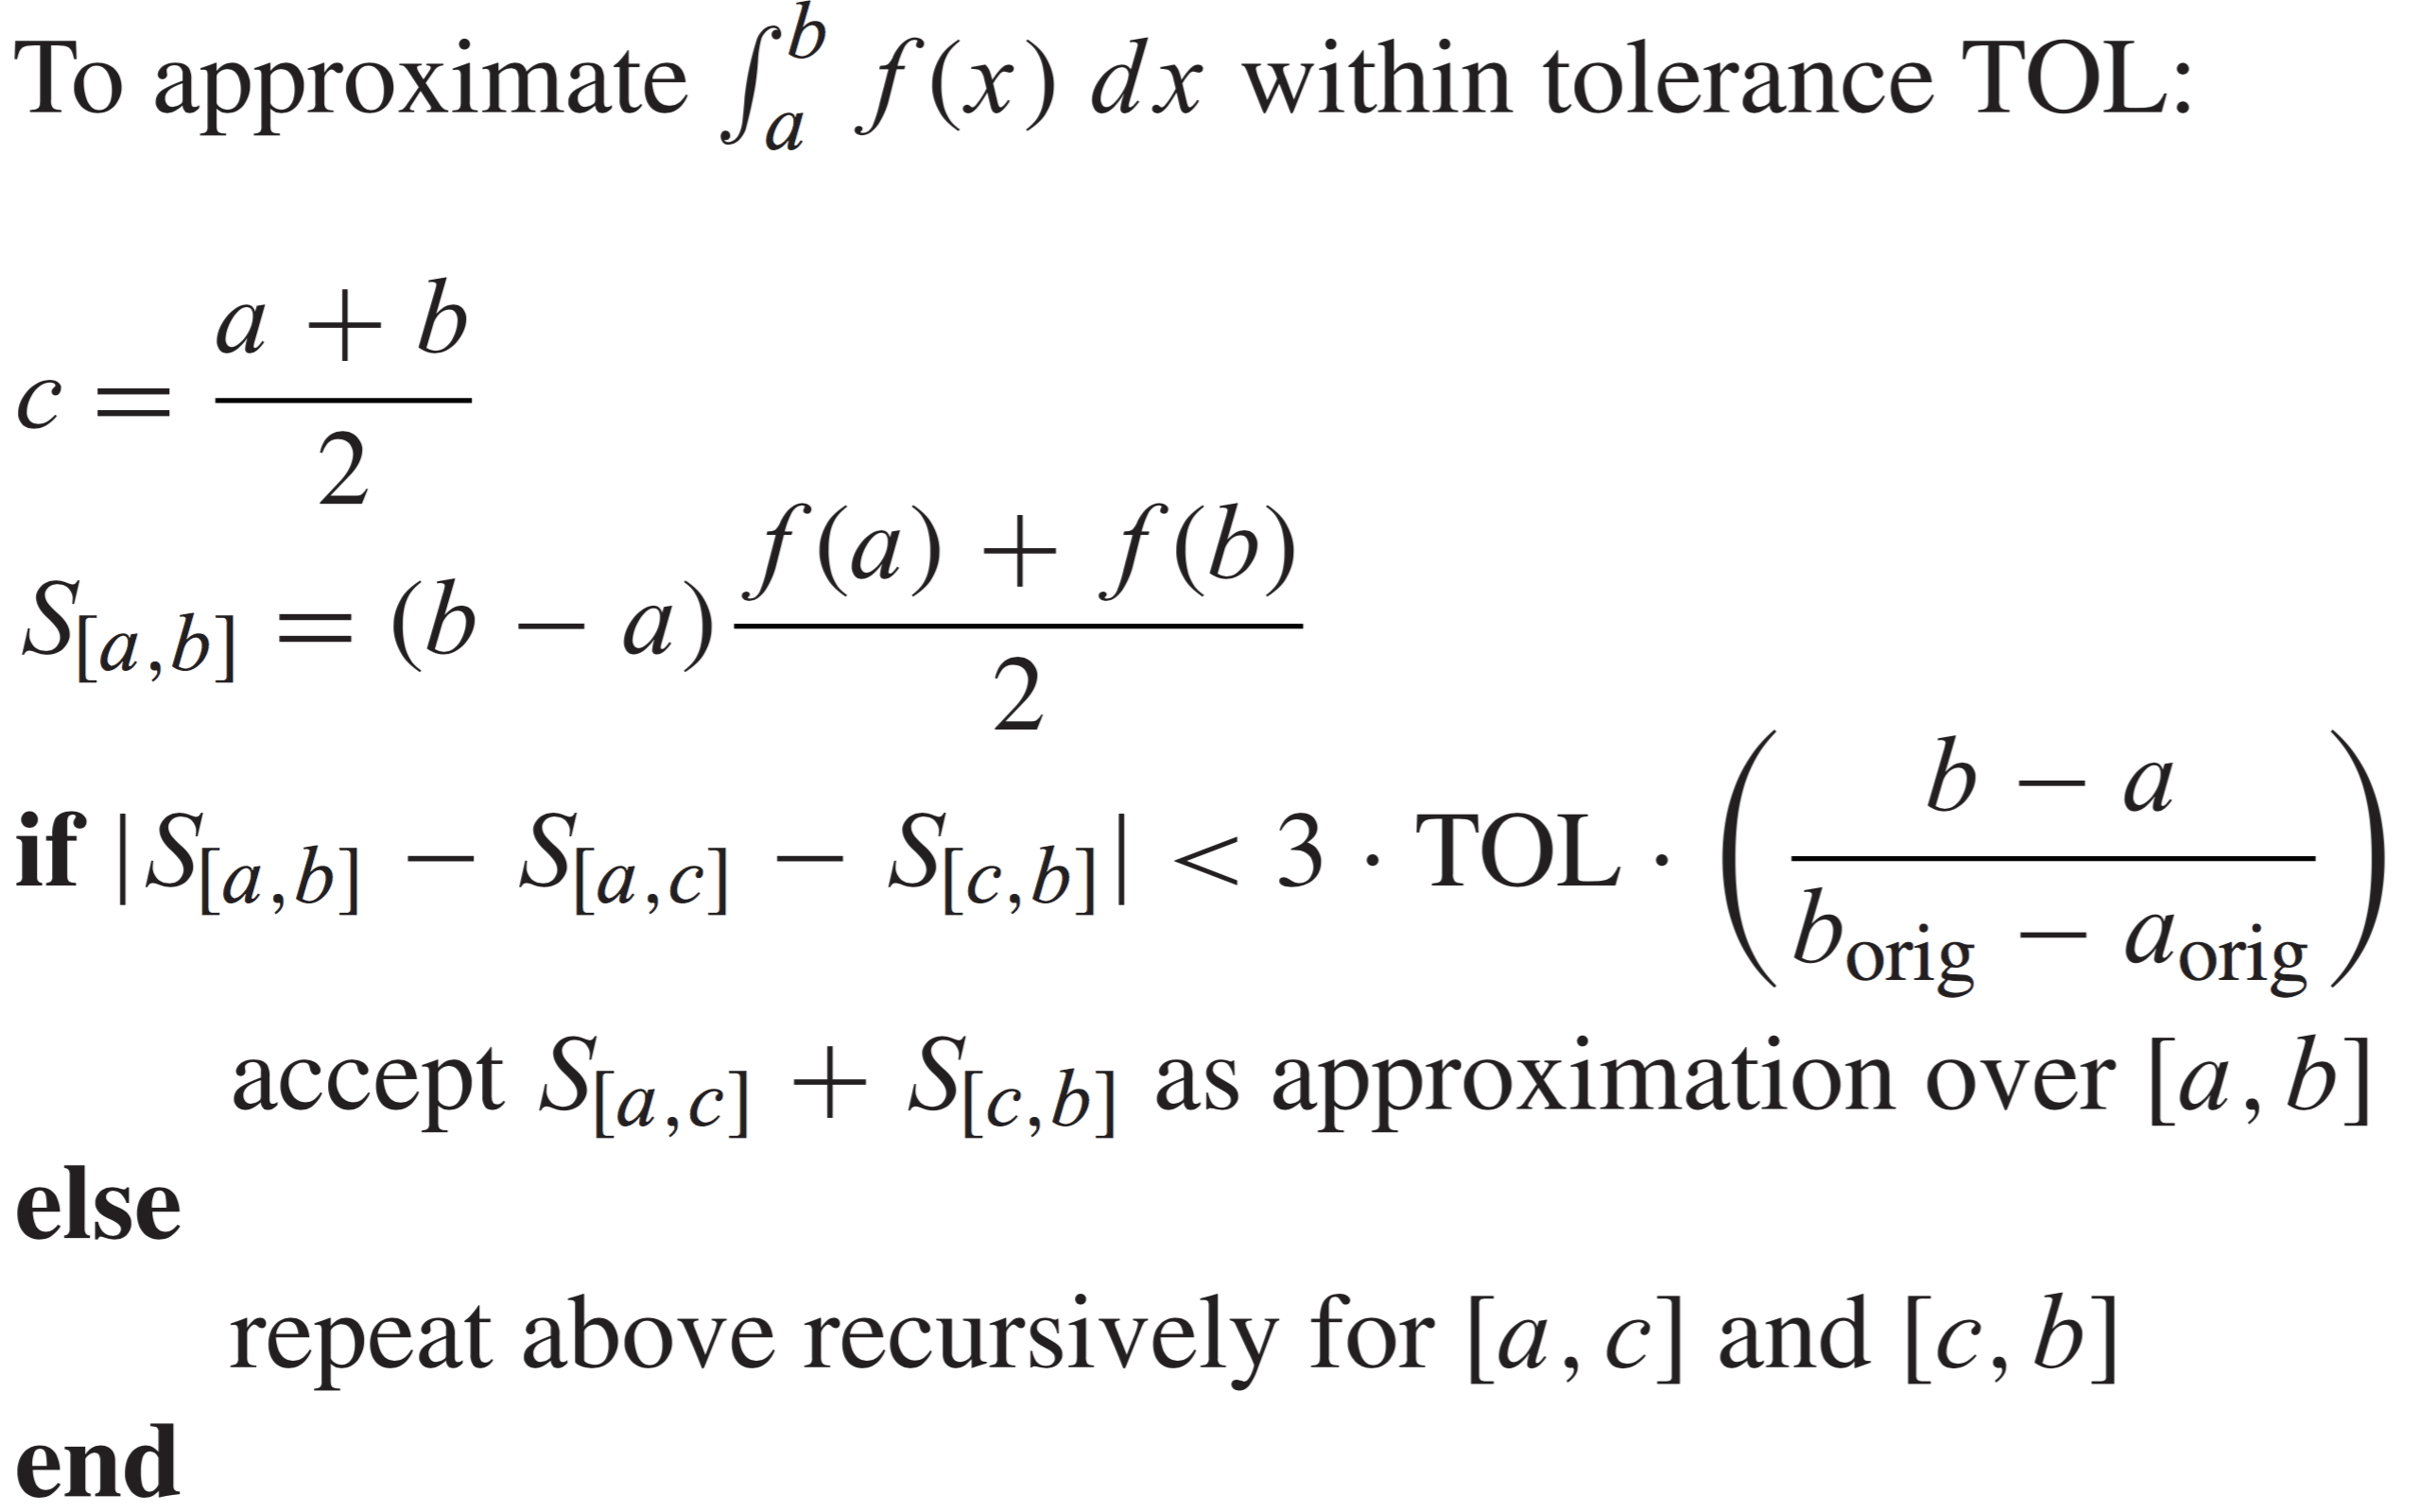
\includegraphics[scale=0.18]{images/adaptive_quadrature.png}
\end{center}

\subsection{Error estimation}
%Do not memorize the exact form of an error estimate for each quadrature, but rather have an idea that they can be derived from either a Taylor series expansion or an interpolation error estimate, when necessary.
Integrate the interpolation error (see "Interpolation Error") or perform a Taylor series expansion and integrate the error term (see "Taylor Method of order $k$"). 